\section{Introduction}
%We employ a search and prune in the graph of state space to learn action classifiers for each query class. At test time given the current state (previous detector responses and the current image) representing by the CNN features of the masked search space, the action classifier will select the most highly scored action. We also incorporate early rejection as an action which will reject further detection if the it isn't likely to contain the query object in the current masks. 

Object detection and segmentation in complex scenes is a central and challenging problem in computer vision and robotics.
%Given an image, for example, Figure~\ref{fig:20Qintro}, our goal is to answer the query: is there a car in the scene, and if yes, to locate it with a bounding box or pixel-wise labels.
This problem is usually tackled by running multiple object detectors exhaustively on densely sampled sliding windows~\cite{felzenszwalb2010object} or category-independent object proposals~\cite{carreira2012cpmc,van2011segmentation,arbelaez2014multiscale}. 
Such methods are time-consuming since they need to evaluate a large number of object hypotheses, and easily introduce false positives if purely considering local appearance cue.
% In addition, due to variations in data distribution, occlusion and viewpoint change, object models may not always capture the appearance of objects and ambiguity arises. 
%In the example of Figure~\ref{fig:20Qintro}, since the viewpoint and the scale of the cars are not similar to those in common training images, it is difficult for the car detector to recognize and locate them.

Instead of checking all hypotheses indiscriminately and exhaustively, humans only look for a set of related objects in a given context~\cite{biederman1982scene, hock1974contextual}. Context information is an effective cue for human to detect low-resolution or small objects in cluttered scenes~\cite{parikh2012exploring}. Many contextual models have been proposed to capture relationships between objects at the semantic level to reduce ambiguities from unreliable detection results~\cite{gould2009decomposing, galleguillos2010context, ladicky2010graph}. %For example, because roads and buildings often co-occur with cars, knowing the existence of these objects can help us infer the locations of cars.  
However, such methods still need to evaluate the high order co-occurrence statistics and spatial relations with \emph{all} other object classes appearing in the scene altogether, some of which may not be informative and even introduce distractions.  

By contrast, human vision is an active process that sequentially samples the optic array in an intelligent, task-specific way~\cite{najemnik2005optimal}~\CXNote{Cite Nature}. Research in neuro-science have revealed that when humans search for a target, those objects that are associative to the query will reinforce attention with the query and weaken recognition of unrelated distractions~\cite{moores2003associative}. 
%This is highly inefficient since many non-informative contextual objects have to be queried. 
For instance, in Figure~\ref{fig:20Qintro}, knowing the top of the scene is sky is not very helpful to distinguish whether there is a car or a boat since both can be under the sky; 
while observing road instead of water in the lower part gives a strong indication of the existence of cars. And then cars are more likely to be found beside the buildings after observing the road. So in order to find the car, human tends to first look for the road, then search around the buildings, instead of looking up to the sky. %And if we know there is road, we do not need to ask about water.
%We note that the set of related object classes and the order of asking questions about them is dynamic given a specific query in the scene and knowledge of previous observations.
This motivates us to raise the question: \textit{can object detection algorithms decide where to look for the object of a query class more accurately by exploring a few related context in a dynamic order like human?}

In this paper, we formulate this process as a Markov Decision Process (MDP), and use imitation learning to learn a context-driven policy that sequentially and dynamically selects the most informative context class to explore and refine the search area for the target. We show our framework in Figure~\ref{fig:flowchart}.  Specifically, like playing a Twenty Question game, at each step the policy makes a decision about which detector of context class to run given the query and responses from previous contextual classifiers. After taking the action to run context classifiers/detectors and observing responses, it then refines the search area for the query object using spatial-aware contextual models. We also incorporate early rejection as an action to avoid further running detection if the policy determines there is a low chance of having the query object in the scene, and this decision can be made even before running any object detectors so it can reduce a large amount of unnecessary computation. Finally, we run the query object detector in the output search area if the policy thinks enough contextual information has been gathered and decides to stop. Object detection experiments in images of complex scenes like Pascal VOC dataset show that our algorithm can produce a search space that's closer to the target object by checking its context, thus significantly reduces the number of object proposals and detector evaluation while maintaining comparable mean average precision (mAP) to exhaustive search. To the best of our knowledge, this is one of the first works to model the challenging task of simultaneous object detection and segmentation in complex real scenes using an imitation learning policy fully driven by semantic context.


\begin{figure*}[htb]
\begin{center}
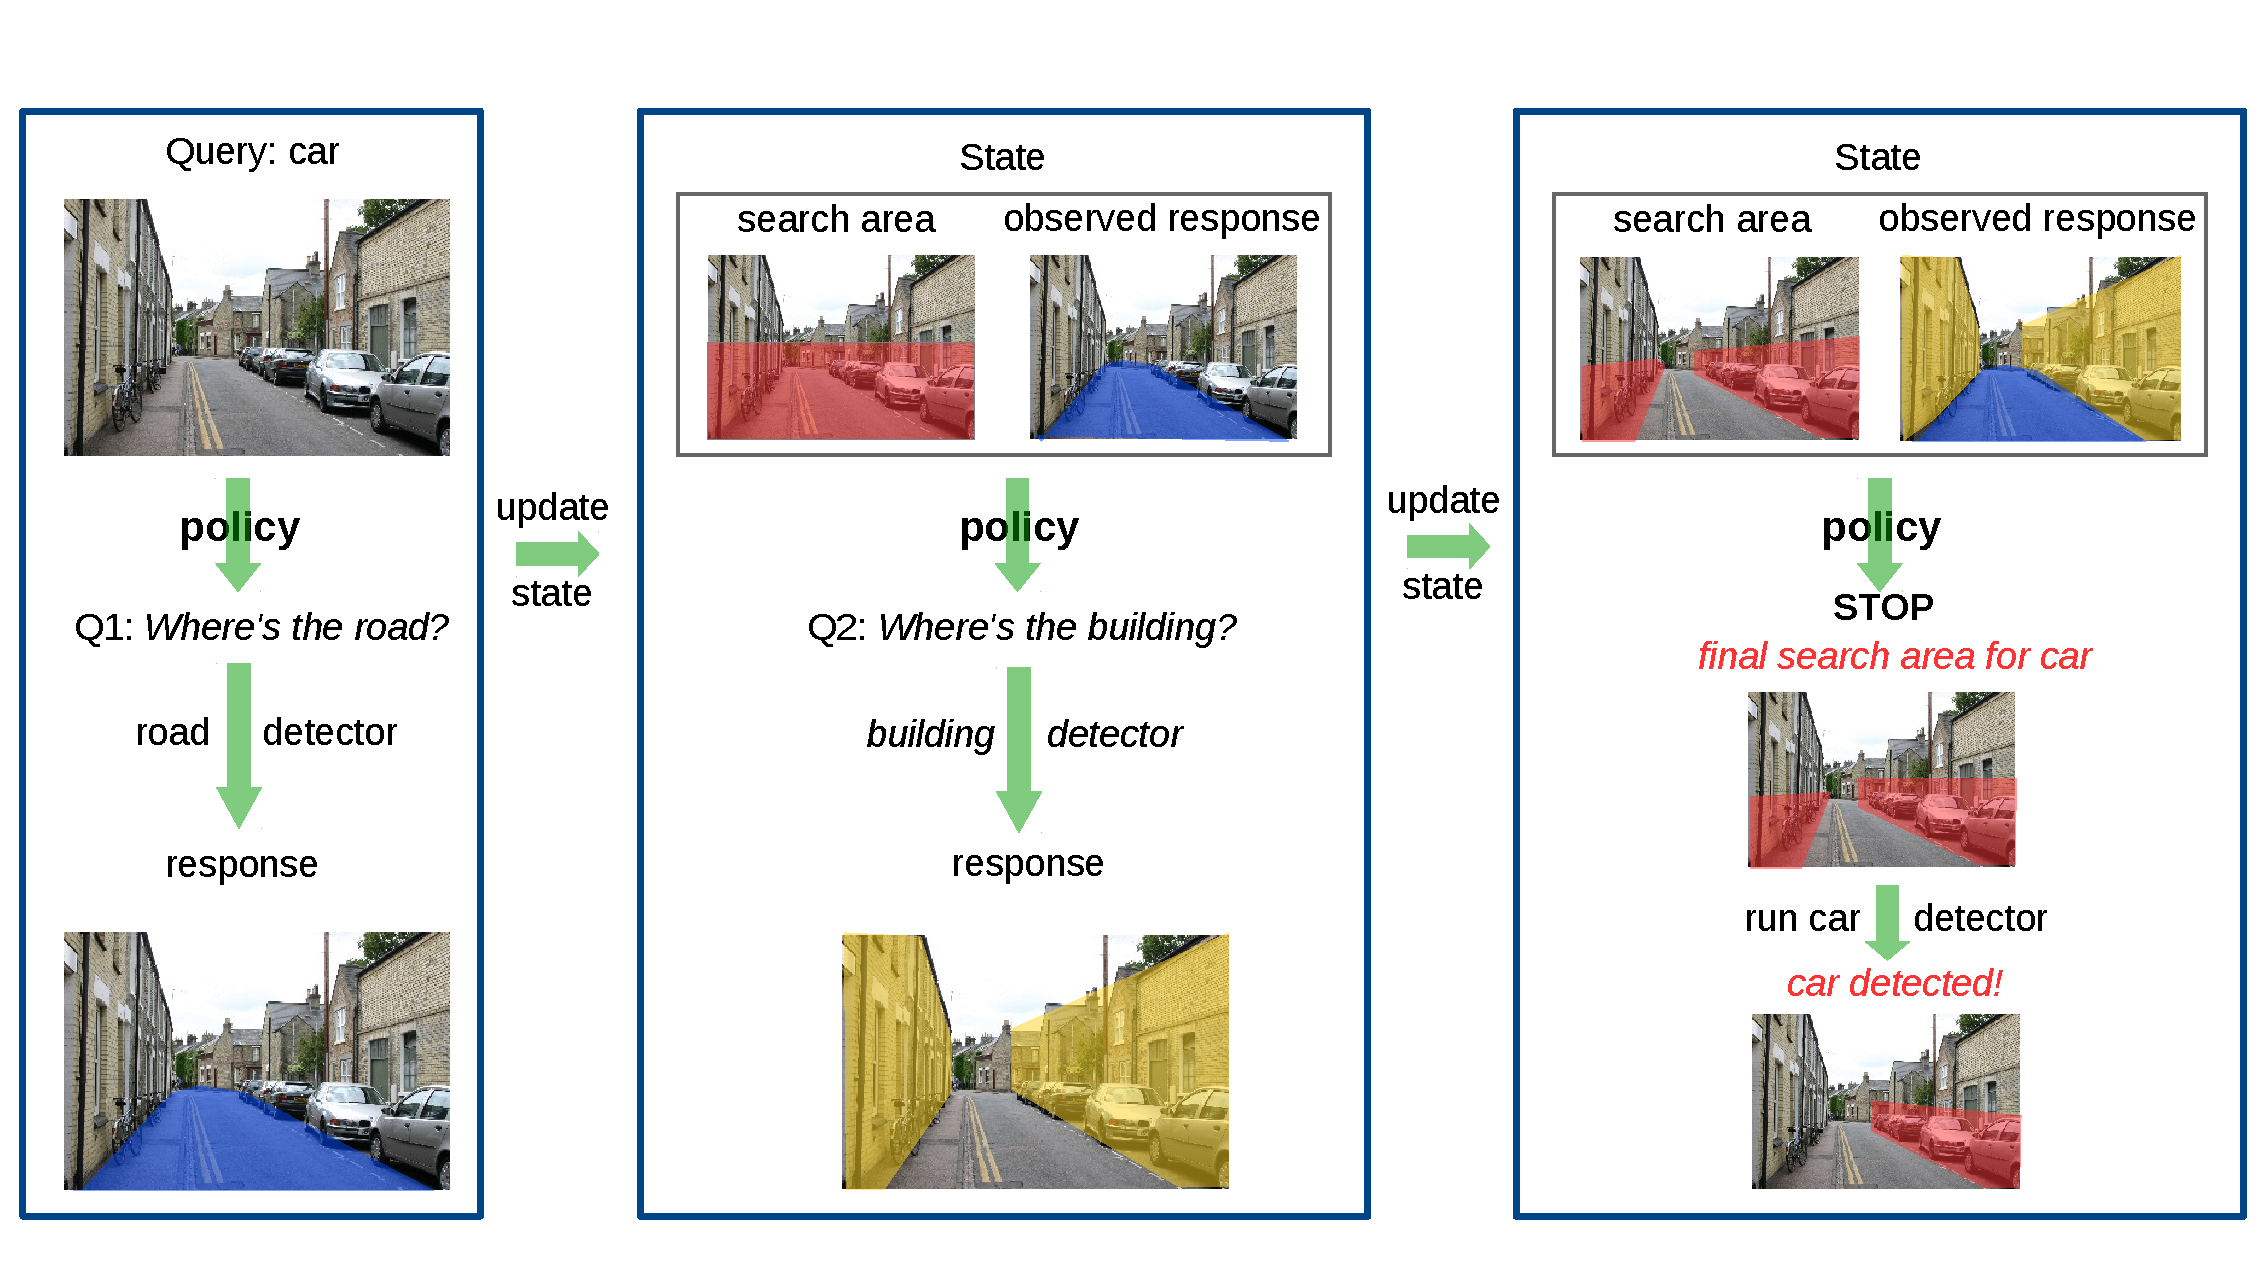
\includegraphics[width=\linewidth]{figures/iccv20q-overview.pdf}
\caption{Illustration of our sequential search for objects in 20 context driven questions.}
\label{fig:20Qintro}
\end{center}
\end{figure*}

% The main contributions of the paper are:
% \HHNote{seems contribution 1 and 2 can be combined, they are both novelty of a new learning algorithm to the problem. e.g., we formulate and learn...}
% \begin{itemize}
% \item a novel formulation of the object detection problem as a Markov Decision Process and a dynamic, closed-loop policy learned by imitation learning to decide which detectors to run next and where to look for the query object iteratively
% \item a general and unified probabilistic framework incorporating responses from multi-class object detectors and contextual classifiers to update the search area for the target
% \item a data-driven context model that not only encodes co-occurrence but also spatial relations by efficient weighted vote maps from exemplars\HHNote{This is not explained before and it's hard to understand here what the context model is}.
% \end{itemize}




